\documentclass[conference,letterpaper]{IEEEtran}
\usepackage[utf8]{inputenc}
\usepackage[T1]{fontenc}
\usepackage[cmex10]{amsmath}
\usepackage{amssymb,amsthm,amsmath}
\usepackage{tikz}
\usepackage{amssymb}
\usetikzlibrary{shapes.geometric}
\usepackage{tikz}
\usepackage{xcolor}
\usepackage{xcolor}
\usepackage{amsmath}
\usetikzlibrary{shapes.geometric}

\begin{document}

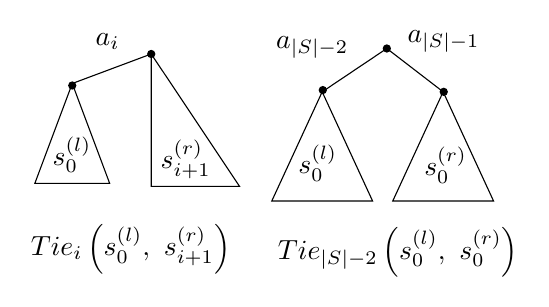
\begin{tikzpicture}[x=0.75pt,y=0.75pt,yscale=-1,xscale=1]

\draw   (113.07,74.05) -- (155.62,137.81) -- (113.07,137.81) -- cycle ;
\draw   (75.02,88.27) -- (93.04,136.37) -- (57,136.37) -- cycle ;
\draw  [line width=3] [line join = round][line cap = round] (75.02,89.23) .. controls (75.02,89.23) and (75.02,89.23) .. (75.02,89.23) ;
\draw  [line width=3] [line join = round][line cap = round] (113.07,74.05) .. controls (113.07,74.05) and (113.07,74.05) .. (113.07,74.05) ;
\draw    (75.02,88.27) -- (113.07,74.05) ;
\draw   (253.72,92.28) -- (278,144.88) -- (229.44,144.88) -- cycle ;
\draw   (195.44,92.28) -- (219.72,144.88) -- (171.16,144.88) -- cycle ;
\draw  [line width=3] [line join = round][line cap = round] (195.73,91.44) .. controls (195.73,91.44) and (195.73,91.44) .. (195.73,91.44) ;
\draw  [line width=3] [line join = round][line cap = round] (254,92.28) .. controls (254,92.28) and (254,92.28) .. (254,92.28) ;
\draw  [line width=3] [line join = round][line cap = round] (226.58,71.4) .. controls (226.58,71.4) and (226.58,71.4) .. (226.58,71.4) ;
\draw    (195.44,92.28) -- (226.58,71.4) ;
\draw    (226.58,71.4) -- (253.72,92.28) ;

% Text Node
\draw (85.04,62.89) node [anchor=north west][inner sep=0.75pt]    {$a_{i}$};
% Text Node
\draw (64.27,112.53) node [anchor=north west][inner sep=0.75pt]    {$s_{0}^{( l)}$};
% Text Node
\draw (116.33,114.13) node [anchor=north west][inner sep=0.75pt]    {$s_{i+1}^{( r)}$};
% Text Node
\draw (53.81,154.67) node [anchor=north west][inner sep=0.75pt]    {$Tie_{i}\left( s_{0}^{( l)} ,\ s_{i+1}^{( r)}\right)$};
% Text Node
\draw (182.66,116.66) node [anchor=north west][inner sep=0.75pt]    {$s_{0}^{( l)}$};
% Text Node
\draw (243.36,117.5) node [anchor=north west][inner sep=0.75pt]    {$s_{0}^{( r)}$};
% Text Node
\draw (172.01,64.47) node [anchor=north west][inner sep=0.75pt]    {$a_{\mid S\mid-2}$};
% Text Node
\draw (235.29,61.64) node [anchor=north west][inner sep=0.75pt]    {$a_{\mid S \mid-1}$};
% Text Node
\draw (172.86,156.25) node [anchor=north west][inner sep=0.75pt]    {$Tie_{\mid S \mid-2}\left( s_{0}^{( l)} ,\ s_{0}^{( r)}\right)$};


\end{tikzpicture}

\end{document}